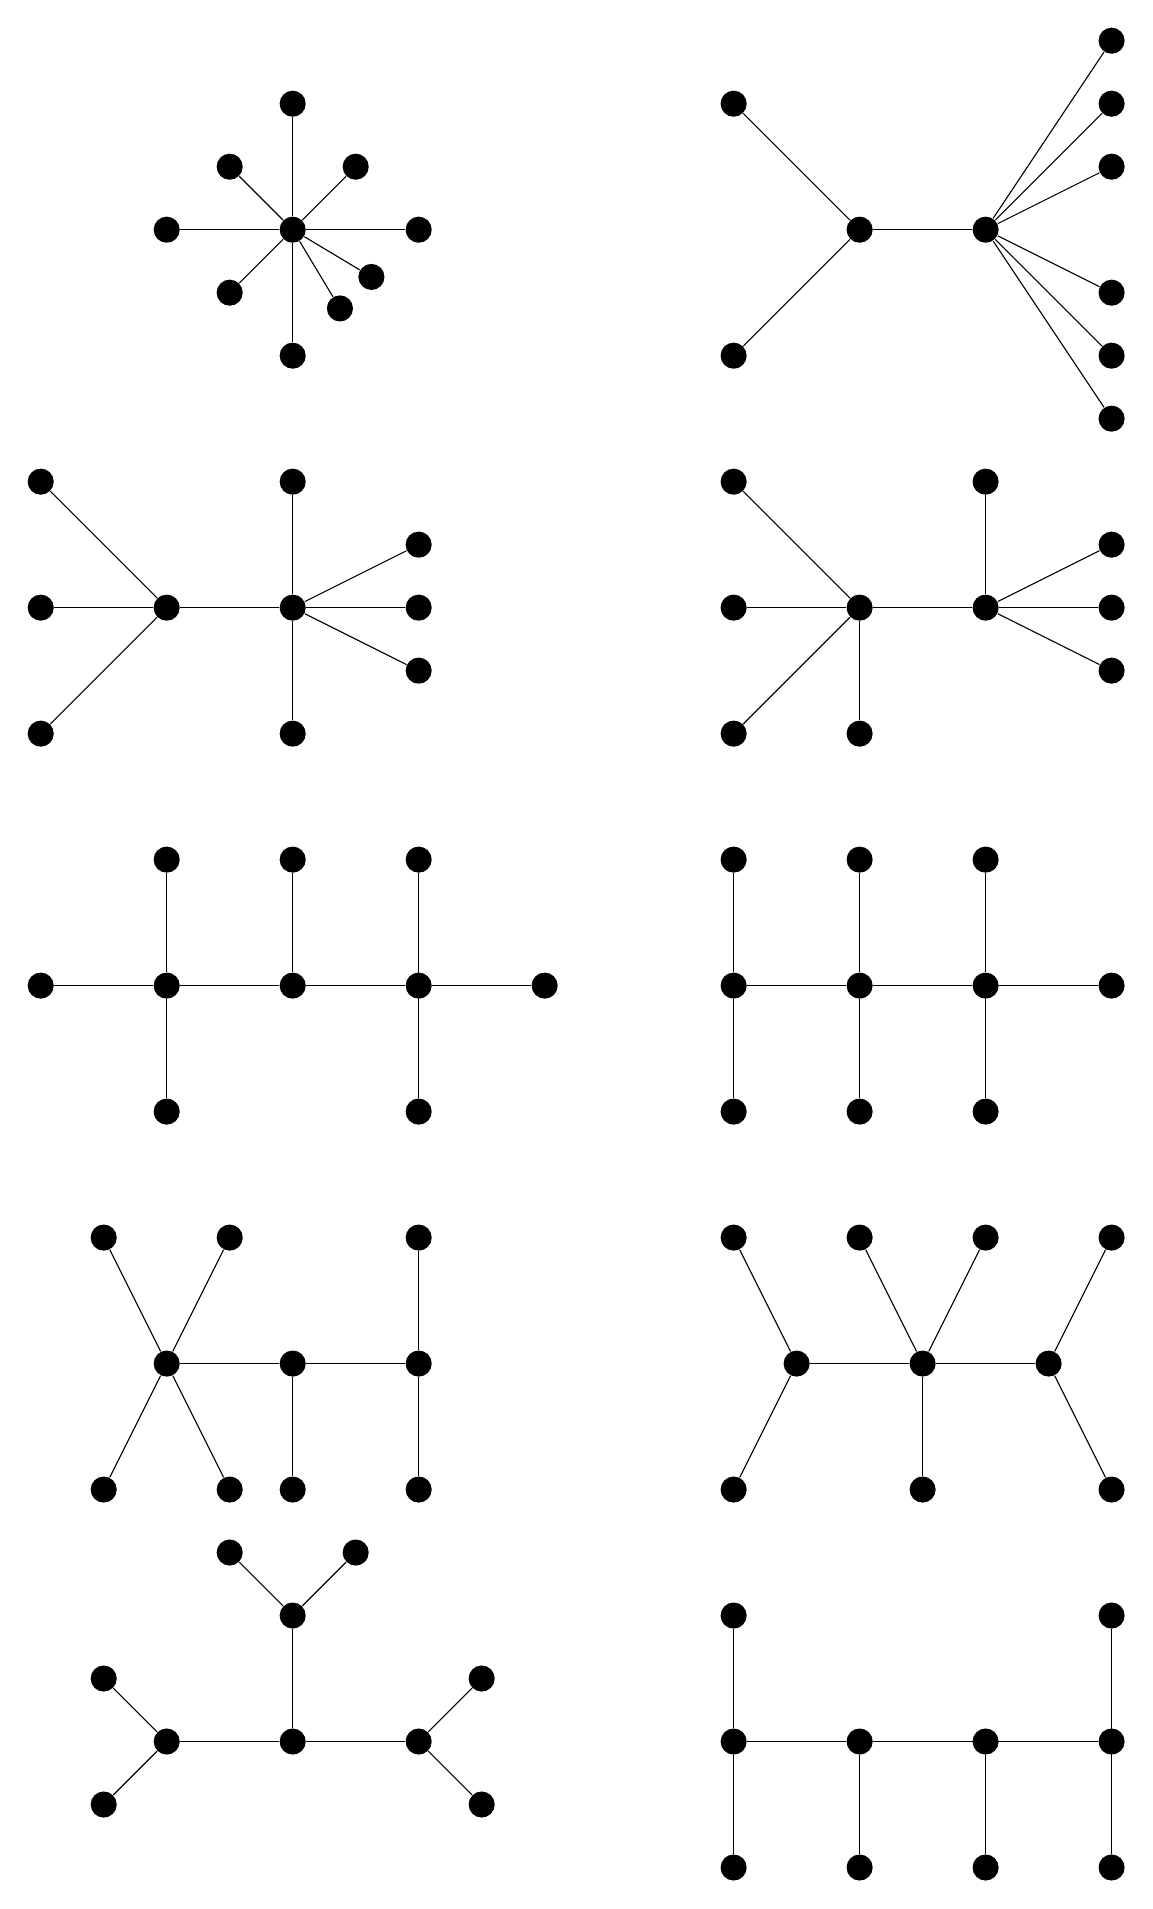
\begin{tikzpicture}[scale = .8]
\node[fill, circle] (A) at (0,0) {}; 
\node[fill, circle] (B) at (2,0) {}; 
\node[fill, circle] (C) at (1,1) {}; 
\node[fill, circle] (D) at (0,2) {}; 
\node[fill, circle] (E) at (-1,1) {}; 
\node[fill, circle] (F) at (-2,0) {}; 
\node[fill, circle] (G) at (-1,-1) {}; 
\node[fill, circle] (H) at (0,-2) {}; 
\node[fill, circle] (I) at (.75,-1.25) {}; 
\node[fill, circle] (J) at (1.25,-.75) {}; 
\draw[-] (A) -- (B);
\draw[-] (A) -- (C);
\draw[-] (A) -- (D);
\draw[-] (A) -- (E);
\draw[-] (A) -- (F);
\draw[-] (A) -- (G);
\draw[-] (A) -- (H);
\draw[-] (A) -- (I);
\draw[-] (A) -- (J);


\begin{scope}[shift={(11,0)}]
\node[fill, circle] (A) at (0,0) {}; 
\node[fill, circle] (B) at (2,3) {}; 
\node[fill, circle] (C) at (2,2) {}; 
\node[fill, circle] (D) at (2,1) {}; 
\node[fill, circle] (E) at (2,-1) {}; 
\node[fill, circle] (F) at (2,-2) {}; 
\node[fill, circle] (G) at (2,-3) {}; 
\node[fill, circle] (H) at (-2,0) {}; 
\node[fill, circle] (I) at (-4,-2) {}; 
\node[fill, circle] (J) at (-4,2) {}; 
\draw[-] (A) -- (B);
\draw[-] (A) -- (C);
\draw[-] (A) -- (D);
\draw[-] (A) -- (E);
\draw[-] (A) -- (F);
\draw[-] (A) -- (G);
\draw[-] (A) -- (H);
\draw[-] (H) -- (I);
\draw[-] (H) -- (J);
\end{scope}
\begin{scope}[shift={(0,-6)}]
\node[fill, circle] (A) at (0,0) {}; 
\node[fill, circle] (B) at (0,2) {}; 
\node[fill, circle] (C) at (2,1) {}; 
\node[fill, circle] (D) at (2,0) {}; 
\node[fill, circle] (E) at (2,-1) {}; 
\node[fill, circle] (F) at (0,-2) {}; 
\node[fill, circle] (G) at (-4,0) {}; 
\node[fill, circle] (H) at (-2,0) {}; 
\node[fill, circle] (I) at (-4,-2) {}; 
\node[fill, circle] (J) at (-4,2) {}; 
\draw[-] (A) -- (B);
\draw[-] (A) -- (C);
\draw[-] (A) -- (D);
\draw[-] (A) -- (E);
\draw[-] (A) -- (F);
\draw[-] (H) -- (G);
\draw[-] (A) -- (H);
\draw[-] (H) -- (I);
\draw[-] (H) -- (J);
\end{scope}
\begin{scope}[shift={(11,-6)}]
\node[fill, circle] (A) at (0,0) {}; 
\node[fill, circle] (B) at (0,2) {}; 
\node[fill, circle] (C) at (2,1) {}; 
\node[fill, circle] (D) at (2,0) {}; 
\node[fill, circle] (E) at (2,-1) {}; 
\node[fill, circle] (F) at (-2,-2) {}; 
\node[fill, circle] (G) at (-4,0) {}; 
\node[fill, circle] (H) at (-2,0) {}; 
\node[fill, circle] (I) at (-4,-2) {}; 
\node[fill, circle] (J) at (-4,2) {}; 
\draw[-] (A) -- (B);
\draw[-] (A) -- (C);
\draw[-] (A) -- (D);
\draw[-] (A) -- (E);
\draw[-] (H) -- (F);
\draw[-] (H) -- (G);
\draw[-] (A) -- (H);
\draw[-] (H) -- (I);
\draw[-] (H) -- (J);
\end{scope}
\begin{scope}[shift={(0,-12)}]
\node[fill, circle] (A) at (0,0) {}; 
\node[fill, circle] (B) at (2,0) {}; 
\node[fill, circle] (C) at (4,0) {}; 
\node[fill, circle] (D) at (-2,0) {}; 
\node[fill, circle] (E) at (-4,0) {}; 
\node[fill, circle] (F) at (-2,-2) {}; 
\node[fill, circle] (G) at (-2,2) {}; 
\node[fill, circle] (H) at (2,2) {}; 
\node[fill, circle] (I) at (2,-2) {}; 
\node[fill, circle] (J) at (0,2) {}; 
\draw[-] (A) -- (B);
\draw[-] (B) -- (C);
\draw[-] (A) -- (D);
\draw[-] (D) -- (E);
\draw[-] (D) -- (F);
\draw[-] (D) -- (G);
\draw[-] (A) -- (J);
\draw[-] (H) -- (I);
\end{scope}
\begin{scope}[shift={(9,-12)}]
\node[fill, circle] (A) at (0,0) {}; 
\node[fill, circle] (B) at (0,2) {}; 
\node[fill, circle] (C) at (0,-2) {}; 
\node[fill, circle] (D) at (-2,0) {}; 
\node[fill, circle] (E) at (-2,-2) {}; 
\node[fill, circle] (F) at (-2,2) {}; 
\node[fill, circle] (G) at (2,0) {}; 
\node[fill, circle] (H) at (2,2) {}; 
\node[fill, circle] (I) at (2,-2) {}; 
\node[fill, circle] (J) at (4,0) {}; 
\draw[-] (A) -- (B);
\draw[-] (A) -- (C);
\draw[-] (A) -- (D);
\draw[-] (D) -- (E);
\draw[-] (D) -- (F);
\draw[-] (A) -- (G);
\draw[-] (G) -- (H);
\draw[-] (G) -- (I);
\draw[-] (G) -- (J);
\end{scope}
\begin{scope}[shift={(0,-18)}]
\node[fill, circle] (A) at (0,0) {}; 
\node[fill, circle] (B) at (2,0) {}; 
\node[fill, circle] (C) at (-2,0) {}; 
\node[fill, circle] (D) at (-1,2) {}; 
\node[fill, circle] (E) at (-1,-2) {}; 
\node[fill, circle] (F) at (-3,2) {}; 
\node[fill, circle] (G) at (-3,-2) {}; 
\node[fill, circle] (H) at (0,-2) {}; 
\node[fill, circle] (I) at (2,-2) {}; 
\node[fill, circle] (J) at (2,2) {}; 
\draw[-] (A) -- (B);
\draw[-] (A) -- (C);
\draw[-] (A) -- (H);
\draw[-] (C) -- (E);
\draw[-] (C) -- (F);
\draw[-] (C) -- (D);
\draw[-] (C) -- (G);
\draw[-] (B) -- (I);
\draw[-] (B) -- (J);
\end{scope}
 \begin{scope}[shift={(10,-18)}]
\node[fill, circle] (A) at (3,2) {}; 
\node[fill, circle] (B) at (1,2) {}; 
\node[fill, circle] (C) at (-3,2) {}; 
\node[fill, circle] (D) at (-1,2) {}; 
\node[fill, circle] (E) at (-2,0) {}; 
\node[fill, circle] (F) at (0,0) {}; 
\node[fill, circle] (G) at (2,0) {}; 
\node[fill, circle] (H) at (3,-2) {}; 
\node[fill, circle] (I) at (0,-2) {}; 
\node[fill, circle] (J) at (-3,-2) {}; 
\draw[-] (A) -- (G);
\draw[-] (B) -- (F);
\draw[-] (C) -- (E);
\draw[-] (D) -- (F);
\draw[-] (E) -- (F);
\draw[-] (F) -- (G);
\draw[-] (H) -- (G);
\draw[-] (F) -- (I);
\draw[-] (E) -- (J);
\end{scope}
 \begin{scope}[shift={(0,-24)}]
\node[fill, circle] (A) at (0,0) {}; 
\node[fill, circle] (B) at (0,2) {}; 
\node[fill, circle] (C) at (-1,3) {}; 
\node[fill, circle] (D) at (1,3) {}; 
\node[fill, circle] (E) at (-2,0) {}; 
\node[fill, circle] (F) at (-3,1) {}; 
\node[fill, circle] (G) at (-3,-1) {}; 
\node[fill, circle] (H) at (2,0) {}; 
\node[fill, circle] (I) at (3,1) {}; 
\node[fill, circle] (J) at (3,-1) {}; 
\draw[-] (A) -- (B);
\draw[-] (B) -- (C);
\draw[-] (B) -- (D);
\draw[-] (A) -- (E);
\draw[-] (E) -- (F);
\draw[-] (E) -- (G);
\draw[-] (A) -- (H);
\draw[-] (H) -- (I);
\draw[-] (H) -- (J);
\end{scope}
 \begin{scope}[shift={(10,-24)}]
\node[fill, circle] (A) at (-3,2) {}; 
\node[fill, circle] (B) at (-3,0) {}; 
\node[fill, circle] (C) at (-3,-2) {}; 
\node[fill, circle] (D) at (-1,0) {}; 
\node[fill, circle] (E) at (-1,-2) {}; 
\node[fill, circle] (F) at (1,0) {}; 
\node[fill, circle] (G) at (1,-2) {}; 
\node[fill, circle] (H) at (3,2) {}; 
\node[fill, circle] (I) at (3,0) {}; 
\node[fill, circle] (J) at (3,-2) {}; 
\draw[-] (A) -- (B);
\draw[-] (B) -- (C);
\draw[-] (B) -- (D);
\draw[-] (D) -- (E);
\draw[-] (D) -- (F);
\draw[-] (F) -- (G);
\draw[-] (D) -- (I);
\draw[-] (H) -- (I);
\draw[-] (H) -- (J);
\end{scope}
\end{tikzpicture}